\documentclass[11pt]{article}

\usepackage{amsmath}
\usepackage{amssymb}
\usepackage{amsfonts}
\usepackage{graphicx}
\usepackage{hyperref}
\usepackage{geometry}
\usepackage{cite}

\geometry{margin=1in}

\title{Gauge-Like Diagnostics on a Kernel-Induced Cochain Operator Architecture}
\author{Tomislav Rupi\'c\\Independent Researcher\\\v{S}ibenik, Croatia}
\date{March 2026}

\begin{document}
\maketitle

\begin{abstract}
We report Stage 8 diagnostics on the previously validated kernel-induced cochain architecture. Earlier work established a scalar Laplacian limit, a low restricted transverse spectral band, structured scalar--transverse deformation response, and a consistent Dirac--Kaehler lift on the same graded complex. The present paper asks a narrower question: whether the existing architecture exhibits field-like and symmetry-like behavior under charge insertion, dispersion, exact-edge perturbation, and loop diagnostics. The committed results show a structured charge-induced edge response, near-$n^{-2}$ scaling of the lowest transverse mode, machine-precision longitudinal decoupling of exact perturbations, smooth nonlocal loop observables, and a local divergence constraint $d_0^{*}A = \rho$ to solver precision in the tested charge-insertion setup. These statements remain strictly operator-level. No claim is made regarding gauge theory, electromagnetism, photons, or quantum field dynamics.
\end{abstract}

\section{Introduction}
The HAOS-IIP numerical program has so far established three architectural layers on a common Gaussian kernel substrate. First, the kernel-induced scalar branch converges to the continuum Laplacian after the appropriate second-moment normalization. Second, the same cochain architecture supports a restricted transverse edge sector with a descending low spectral band and continuum-like scaling. Third, the graded cochain complex admits a consistent Dirac--Kaehler lift in two and three dimensions, with the algebraic identity
\begin{equation}
D_{DK}^2 = \Delta_H
\end{equation}
holding grade by grade to numerical precision on the tested periodic complexes.

Those results establish operator existence and algebraic consistency. The next question is behavioral rather than architectural: what diagnostics do the already validated operators produce when they are treated as field-like objects? The present paper addresses that question through four committed Stage 8 diagnostics and one refinement. The tests are deliberately narrow. They ask whether the existing architecture exhibits (i) structured response to a localized scalar source, (ii) continuum-like scaling of the low transverse branch, (iii) redundancy under exact edge shifts, (iv) stable loop observables, and (v) a local divergence constraint analogous to a Gauss-type law.

The interpretation boundary is unchanged from the earlier papers. This is an operator-level numerical study only. The purpose is not to claim gauge theory, Maxwell dynamics, photons, or particle content, but to document whether the validated scalar, transverse, and cochain operators display field-like and symmetry-like behavior on the frozen substrate.

\section{Frozen Architecture and Diagnostic Scope}
No operators are modified in this paper. The diagnostics use the previously validated kernel-induced scalar operator, the edge Hodge operator
\begin{equation}
L_1 = d_0 d_0^{*} + d_1^{*} d_1,
\end{equation}
and the restricted transverse sector obtained from the cochain decomposition
\begin{equation}
C^1 = \operatorname{im} d_0 \oplus \mathcal{H}^1 \oplus \operatorname{im} d_1^{*}.
\end{equation}
The transverse operator tested in Stages 3, 4, and 8 is
\begin{equation}
T = d_1^{*} d_1\big|_{\ker(d_0^{*}) \cap (\mathcal{H}^1)^\perp}.
\end{equation}
All Stage 8 diagnostics therefore probe the behavior of already validated operators on the frozen periodic cochain architecture. They do not introduce a new action, new field content, or new first-order lift.

All numerical datasets cited below correspond to stamped artifacts committed in the repository. The text is tied to those committed outputs rather than to uncommitted exploratory runs.

\section{Charge Insertion and Local Source Constraint}
The first diagnostic inserts a mean-zero scalar source $\rho$ on $\Omega^0$ and solves
\begin{equation}
L_0 \phi = \rho,
\end{equation}
then constructs the induced edge field
\begin{equation}
A = d_0 \phi.
\end{equation}
The original Stage 8A run at $n=16$ already showed a smooth radial decay profile and stable shell flux balance, with a discrete conservation residual of $2.72 \times 10^{-15}$. The field magnitude decays approximately as $r^{-2.60}$ over the fitted range, which is steeper than the continuum Coulomb value but clearly structured rather than noisy.

The stronger result comes from the Stage 8.5A refinement, which compares the induced field directly with the local divergence constraint
\begin{equation}
G = d_0^{*} A.
\end{equation}
Across $n=12,16,20$, the best-fit relation
\begin{equation}
G \approx c\,\rho
\end{equation}
returns
\begin{equation}
c = 1.000000
\end{equation}
for every tested size, with correlation coefficient exactly $1.0$ and relative $L^2$ residuals at the level of $10^{-15}$. The corresponding $L^{\infty}$ residuals are also at the level of $10^{-15}$. In the integrated divergence-theorem form, the maximum signed shell-flux mismatch decreases from $8.70\times 10^{-3}$ at $n=12$ to $3.13\times 10^{-3}$ at $n=20$.

This is the strongest local Stage 8 result. The architecture is not merely producing a smooth field-like response to a source. In the tested setup it satisfies the discrete constraint
\begin{equation}
d_0^{*}A = \rho
\end{equation}
to solver precision, with the integrated flux mismatch refining in the expected direction. This identity is not imposed as an external constraint; it arises from the interaction of the validated scalar operator and the discrete exterior calculus on the kernel substrate.

\begin{figure}[t]
\centering
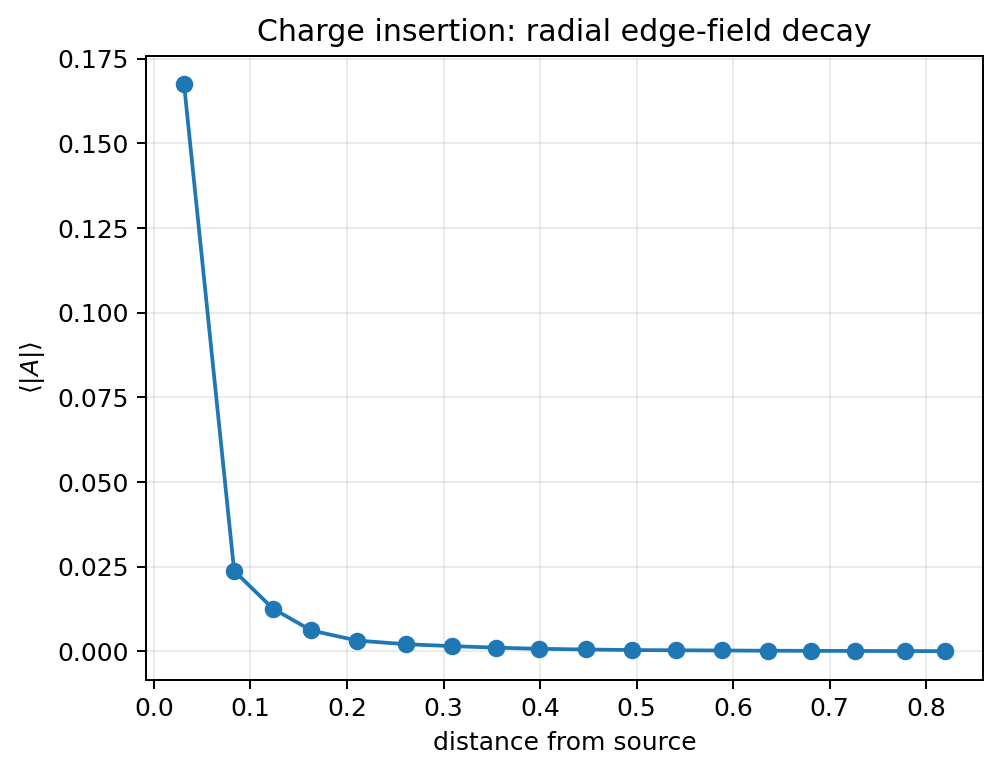
\includegraphics[width=0.32\linewidth]{../plots/20260310_191933_charge_radial_decay.png}
\hfill
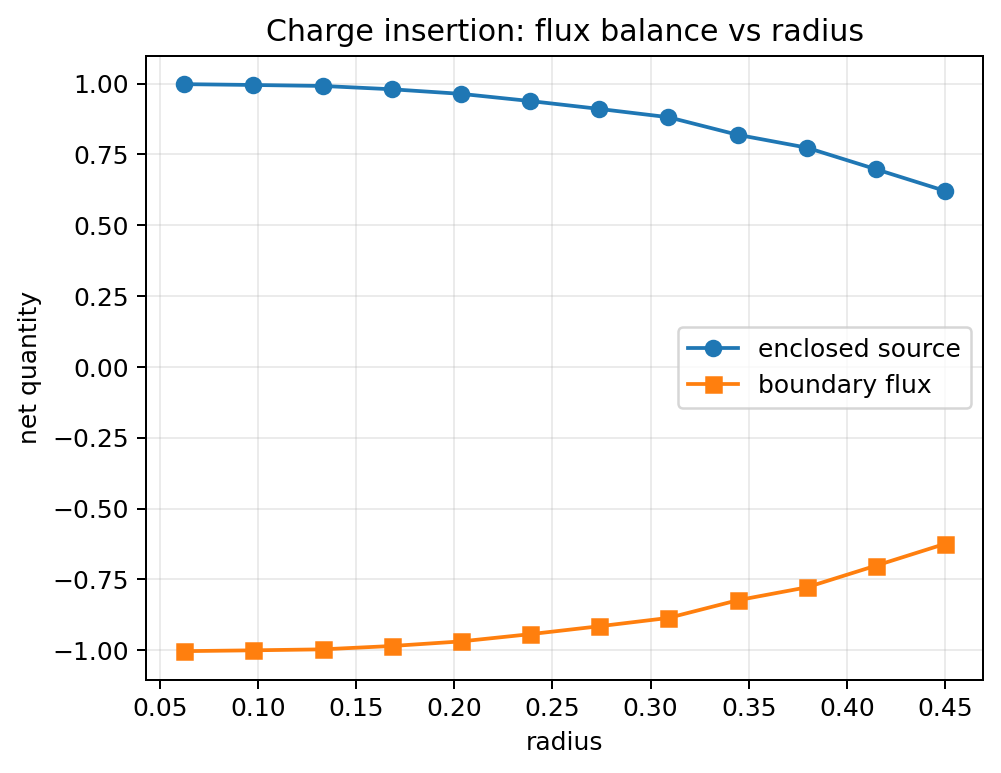
\includegraphics[width=0.32\linewidth]{../plots/20260310_191933_charge_flux_balance.png}
\hfill
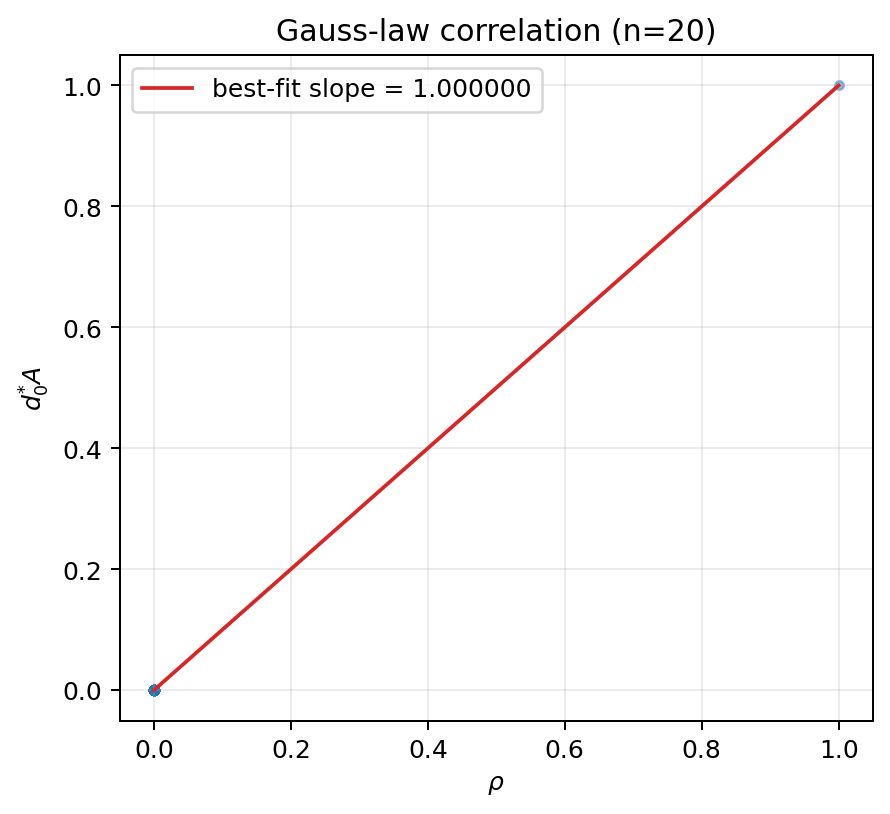
\includegraphics[width=0.32\linewidth]{../plots/20260310_192921_gauss_correlation.png}
\caption{Stage 8 charge-insertion diagnostics. Left: radial decay of the induced edge-field magnitude from the original Stage 8A run. Center: shell flux balance versus radius for the same run. Right: Stage 8.5A correlation between $d_0^{*}A$ and $\rho$ on the largest tested grid, with unit fitted slope.}
\label{fig:charge-gauss}
\end{figure}

\section{Transverse Dispersion and Scaling}
The dispersion diagnostics examine whether the low restricted transverse band behaves like a continuum propagation sector. The original Stage 8B run used $n=12,16,20$ and found that the lowest transverse eigenvalue scales with an almost constant $n^2\lambda_1$ product,
\begin{equation}
37.92,\ 38.59,\ 38.91,
\end{equation}
while the mean divergence norm at the largest size remains at $1.51\times 10^{-16}$. This is the strongest part of the dispersion evidence: the lowest band edge follows the expected Laplacian-type finite-size scaling. By contrast, the direct fit to a coarse momentum model,
\begin{equation}
\lambda \approx c_{\mathrm{eff}} |k|^2 + m_{\mathrm{eff}},
\end{equation}
remains only moderate in quality, with $R^2 \approx 0.64$ at $n=20$.

The refinement run extends the size scan to $n=24$ and sharpens the scaling statement. The lowest-mode data become
\begin{equation}
n^2\lambda_1 = 38.5949,\ 38.9108,\ 39.0834
\end{equation}
for $n=16,20,24$, and the fitted power law
\begin{equation}
\lambda_1(n) \approx 35.4072\, n^{-1.9688}
\end{equation}
reaches $R^2 = 0.999997$. This is very close to the $n^{-2}$ scaling expected for a low continuum Laplacian mode on a finite domain. The direct momentum fit remains only moderate even in the refinement run, with $R^2 \approx 0.674$ at $n=24$, so the dispersion evidence is substantially stronger in the finite-size scaling than in the present momentum assignment.

The bounded interpretation is therefore specific: the low transverse band exhibits strong continuum-like scaling of its floor, while the direct reconstruction of $\lambda(|k|)$ is still limited by a crude momentum assignment. The direct momentum assignment remains coarse; the scaling of the lowest mode is the more reliable continuum indicator in the present data.

\begin{figure}[t]
\centering
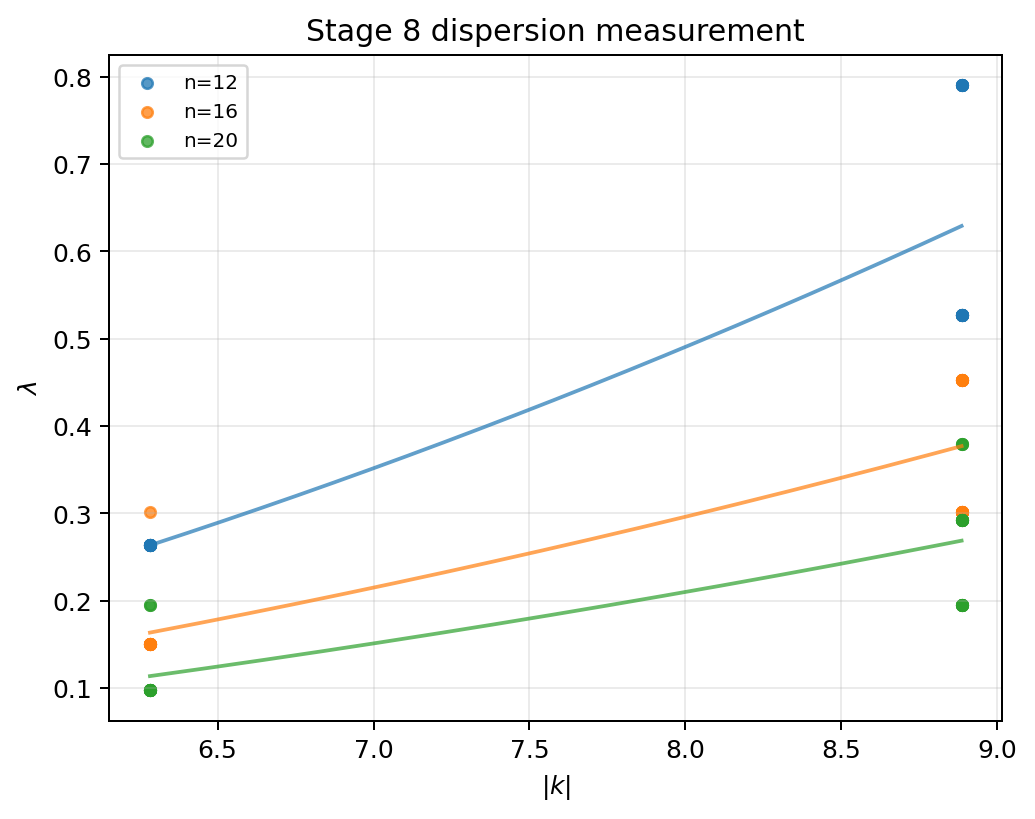
\includegraphics[width=0.32\linewidth]{../plots/20260310_192104_dispersion_curve.png}
\hfill
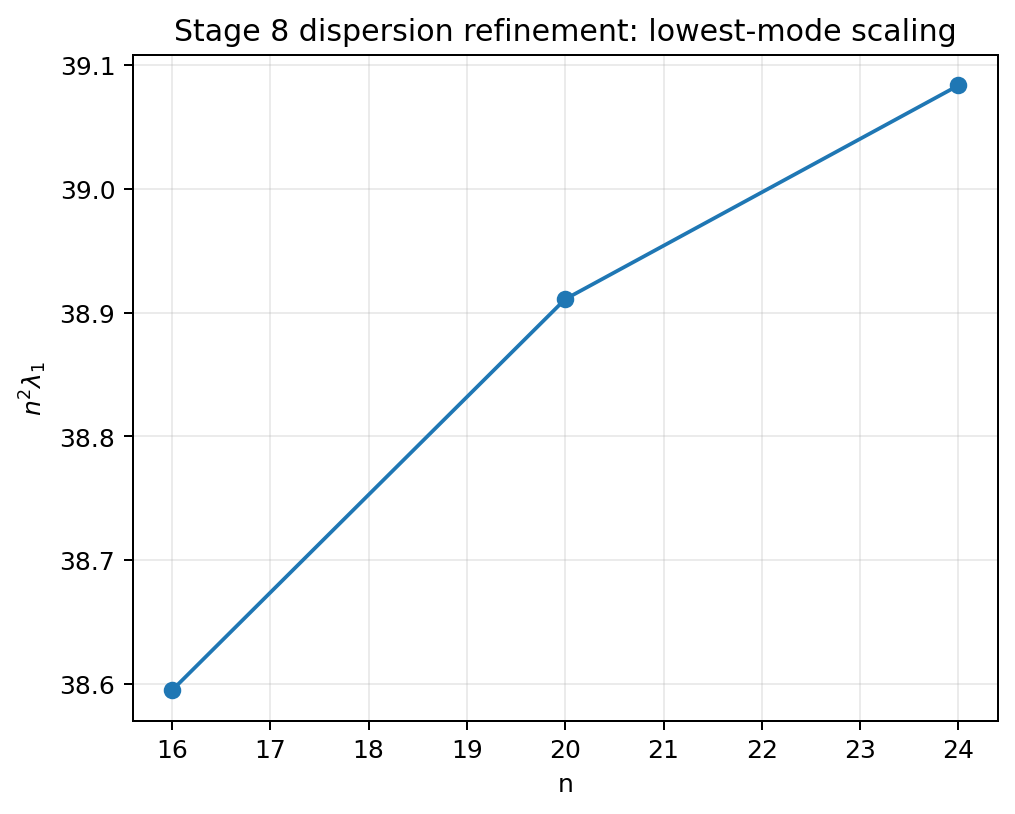
\includegraphics[width=0.32\linewidth]{../plots/20260310_194540_dispersion_refinement_n2lambda.png}
\hfill
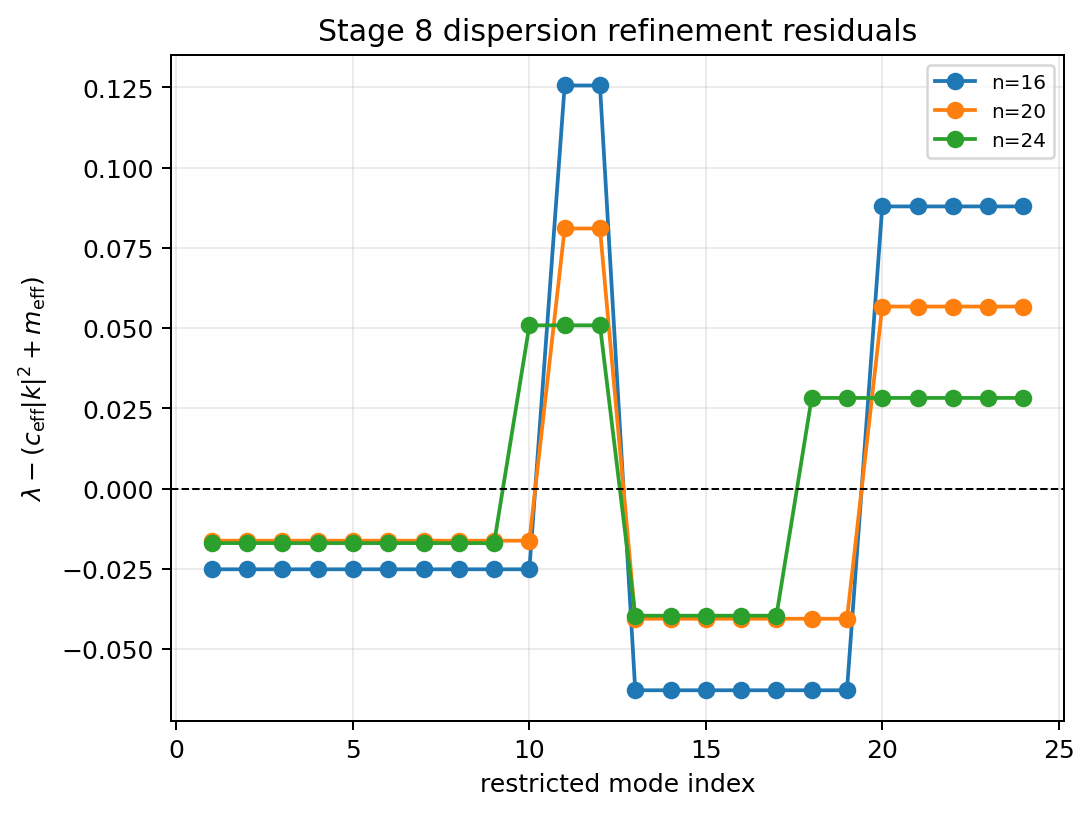
\includegraphics[width=0.32\linewidth]{../plots/20260310_194540_dispersion_refinement_residuals.png}
\caption{Stage 8 dispersion diagnostics. Left: original Stage 8B low-band dispersion plot for $n=12,16,20$. Center: refinement of the lowest-mode scaling through the near-constant plateau in $n^2\lambda_1$ for $n=16,20,24$. Right: residuals of the direct momentum fit in the refinement run.}
\label{fig:dispersion}
\end{figure}

\section{Longitudinal Decoupling}
The third diagnostic tests the response of restricted transverse observables under the addition of exact edge components,
\begin{equation}
A' = A + d_0\varphi.
\end{equation}
This is the cleanest symmetry-like probe in the current architecture. On the $n=16$ periodic complex, the Stage 8C run compares the restricted projection, coexact energy, spectral weights, and divergence-free projection for amplitudes $\alpha = 0, 0.25, 0.5, 1.0, 2.0$ multiplying a smooth exact perturbation.

The result is numerically decisive. The projection and divergence-free residuals remain at the level of $10^{-14}$, the spectral-weight residuals are at the level of $10^{-16}$, and the coexact-energy residual is exactly zero for all tested amplitudes. In other words, within numerical precision the restricted transverse observables are invariant under addition of pure exact components.

This is stronger than a spectral coincidence. It demonstrates a redundancy structure at the level of the tested observables. The correct bounded statement is the one already used in the repository log: the longitudinal-decoupling diagnostic is consistent with redundancy of exact perturbations at the restricted transverse level.

\begin{figure}[t]
\centering
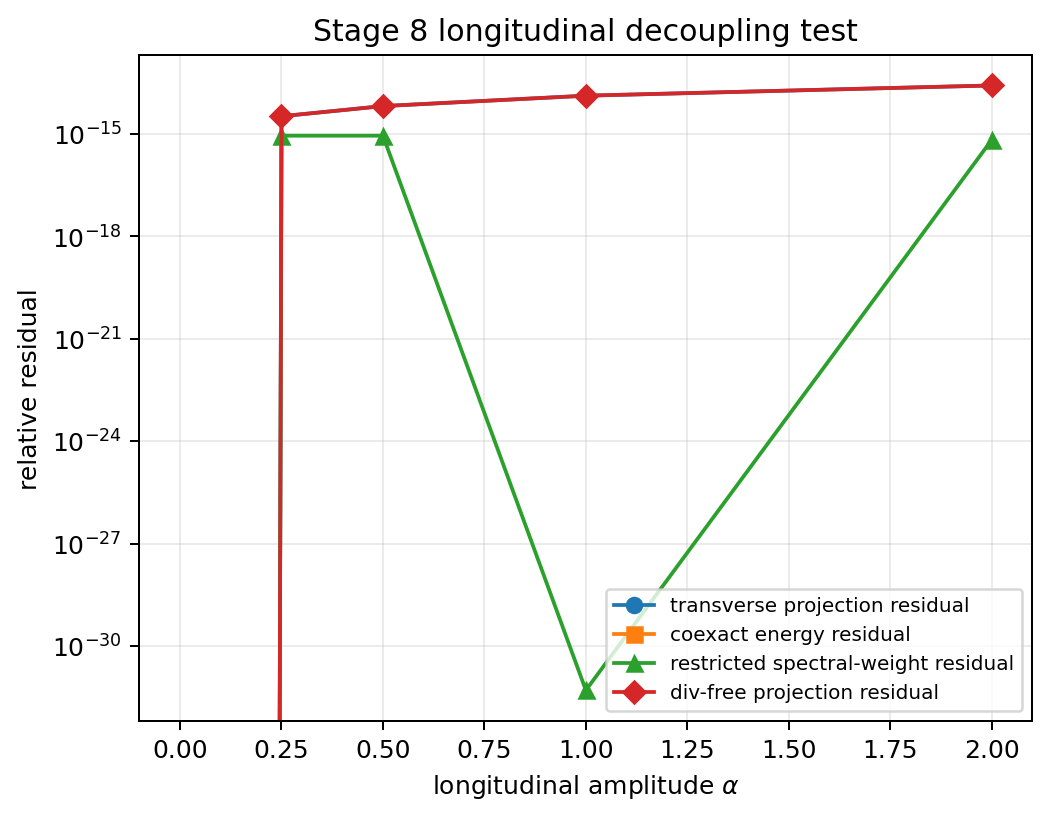
\includegraphics[width=0.55\linewidth]{../plots/20260310_192113_decoupling_residuals.png}
\caption{Stage 8C longitudinal-decoupling residuals on the $n=16$ periodic complex. Projection, spectral, and divergence-free residuals remain at numerical precision while the coexact energy is unchanged.}
\label{fig:decoupling}
\end{figure}

\section{Loop Response Diagnostics}
The final Stage 8 block probes nonlocal behavior through square-loop functionals computed from the lowest restricted transverse mode on the periodic architecture. The original Stage 8D run used loop sides $1$ through $4$ and found a smooth increase in the mean absolute loop response. Over that limited range, power-law fits against loop perimeter and loop area are both excellent,
\begin{equation}
R^2 = 0.9998,
\end{equation}
with exponents $1.93$ in the perimeter parametrization and $0.97$ in the area parametrization. Because square loops tie perimeter and area algebraically, that short scan cannot distinguish a unique scaling class.

The refinement extends the loop range to sides $1$ through $8$. The response remains smooth and monotone, with values
\begin{equation}
0.00287,\ 0.01126,\ 0.02456,\ 0.04162,\ 0.06125,\ 0.08158,\ 0.10115,\ 0.11773.
\end{equation}
The extended fits become
\begin{equation}
\text{perimeter exponent} = 1.8039,
\qquad
\text{area exponent} = 0.9019,
\end{equation}
with the same $R^2 = 0.9961$ in both parametrizations. This sharpened scan strengthens the statement that the loop observable is stable and nonlocal, but it still does not distinguish perimeter from area scaling on this square-loop family alone.

That is the correct reading for the paper: the architecture supports a smooth loop observable whose scaling is stable under range extension, but the scaling class remains ambiguous in the present geometry. For the square-loop family studied here, perimeter and area scaling remain algebraically coupled over the tested range.

\begin{figure}[t]
\centering
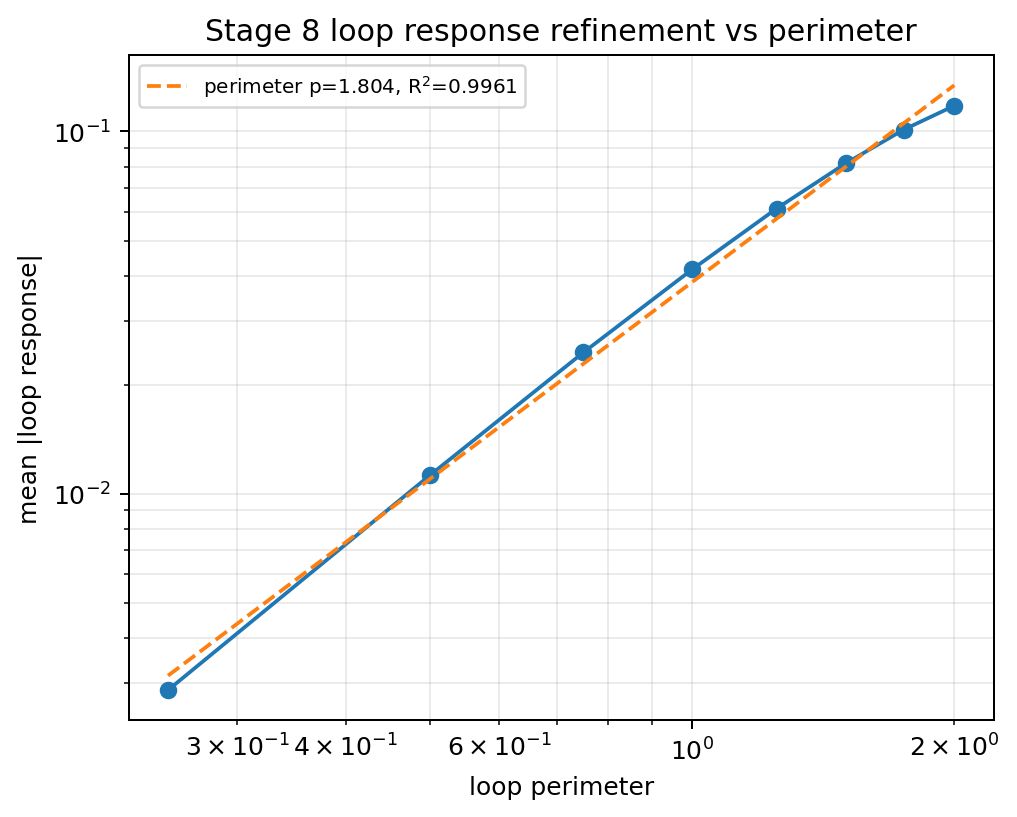
\includegraphics[width=0.48\linewidth]{../plots/20260310_194548_loop_response_extended_perimeter.png}
\hfill
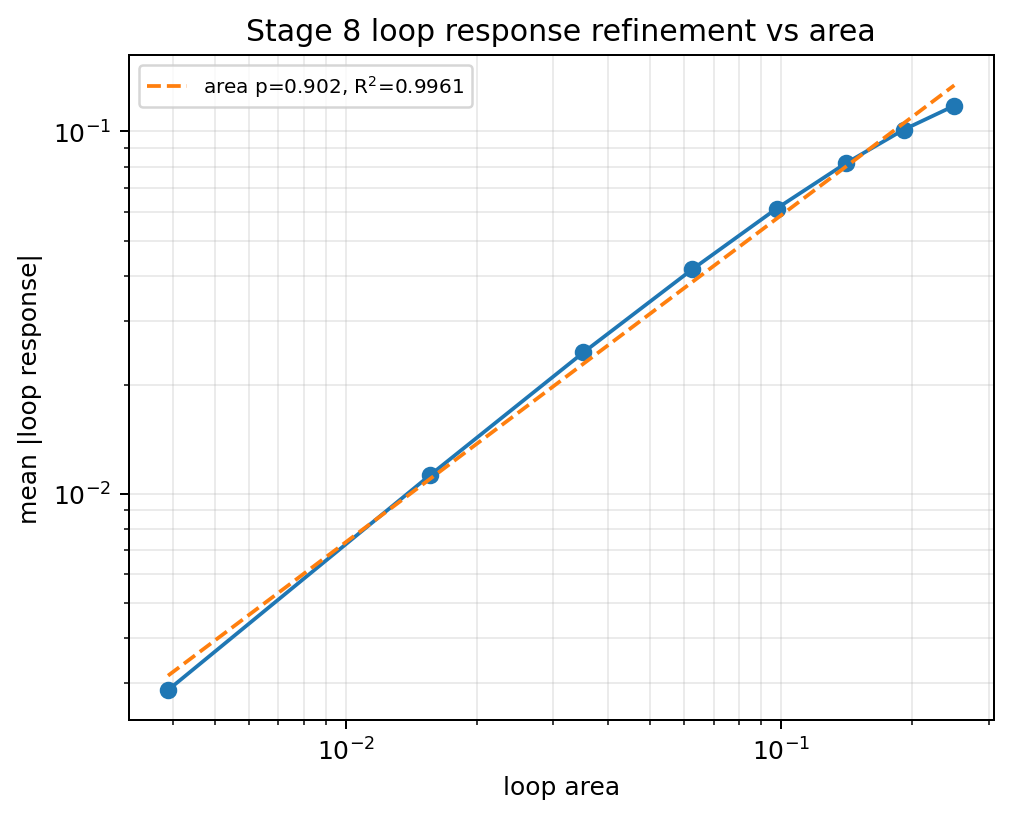
\includegraphics[width=0.48\linewidth]{../plots/20260310_194548_loop_response_extended_area.png}
\caption{Extended Stage 8D loop-response diagnostics for square loops of side $1$ through $8$. The observable remains smooth and well fit in both the perimeter and area parametrizations, but the present loop family does not yet separate those two scaling classes.}
\label{fig:loop-response}
\end{figure}

\section{Interpretation Boundary}
The results reported here remain strictly operator-level. The charge-insertion path shows a structured induced edge response and, in the refined diagnostic, an exact local divergence constraint on the tested periodic complex. The transverse band shows strong finite-size scaling of its lowest mode and machine-precision invariance under exact shifts of the edge field. The loop observable shows stable nonlocal scaling under range extension.

These results do not establish gauge theory, electromagnetism, photons, fermions, or quantum field dynamics. They show only that the previously validated kernel-induced cochain architecture exhibits field-like response, redundancy-like behavior, and nonlocal loop structure under the committed Stage 8 diagnostics.

\section{Conclusion}
This paper marks the transition from operator existence to operator behavior in the HAOS-IIP program. Earlier stages established the scalar branch, the restricted transverse branch, scalar--transverse deformation response, and the Dirac--Kaehler lift on the same cochain architecture. The present Stage 8 diagnostics ask what the already validated operators do when tested as field-like objects rather than only as abstract spectra.

The strongest new results are local. The induced edge field from a scalar source satisfies
\begin{equation}
d_0^{*}A = \rho
\end{equation}
to solver precision in the tested setup, and the restricted transverse observables remain invariant under exact perturbations to numerical precision. These two diagnostics provide the clearest structural signals in the current run. The remaining diagnostics are weaker but still informative: the transverse floor now exhibits near-$n^{-2}$ scaling through the refinement scan, and the loop observable remains smooth and stable over an extended range, although its scaling class is not yet uniquely resolved.

The narrow conclusion is that the frozen architecture supports structured field-like response, continuum-like scaling of the low transverse floor, exact longitudinal decoupling at the restricted level, stable loop observables, and a local divergence constraint consistent with a Gauss-like law. This remains an operator-level numerical statement only. Future refinement can focus on larger lattice sizes for the dispersion diagnostic and more discriminating loop families for the nonlocal scaling test.

\begin{thebibliography}{9}

\bibitem{paper1}
Tomislav Rupi\'c,
\newblock \emph{Kernel-Induced Operator Architecture and the Emergence of a Transverse Spectral Band on Discrete Substrates},
\newblock HAOS-IIP preprint, 2026.

\bibitem{paper2}
Tomislav Rupi\'c,
\newblock \emph{Continuum Reconstruction and Scalar-Transverse Coupling in Kernel-Induced Operator Systems},
\newblock HAOS-IIP preprint, 2026.

\bibitem{paper3}
Tomislav Rupi\'c,
\newblock \emph{Dirac-Kaehler Factorization on a Validated Cochain Operator Architecture},
\newblock HAOS-IIP preprint, 2026.

\bibitem{repo}
Tomislav Rupi\'c,
\newblock \emph{HAOS-IIP Repository and Stamped Numerical Artifacts},
\newblock GitHub repository, \url{https://github.com/tomislavrupic}.

\end{thebibliography}

\section*{Project Resources}
Project website: \url{https://tomislav-rupic.com/}

Code repository: \url{https://github.com/tomislavrupic}

Archived release (Zenodo DOI): \url{https://doi.org/10.5281/zenodo.18938323}

\end{document}
